
%%
%\begin{frame}
%	\frametitle{Marc Rußwurm}
%	
%	\begin{columns}
%		\column{.66\textwidth}
%			\uncover<2->{
%				\begin{itemize}
%					\item born in raised in Bavaria, Germany.
%					\item recently finished Master Geodesy \& Geoinformation @ TU Munich
%					\item now started PhD @ TUM/DLR \\ Chair of Remote Sensing Technology
%					\item member Computer Vision Research Group of the Chair
%				\end{itemize}
%			}
%			\uncover<3->{
%				\vspace{1em}
%				scientific interests
%				\begin{itemize}
%					\item multi-temporal EO
%					\item time series with Recurrent Nets
%					\item natural language processing $\rightarrow$ EO
%				\end{itemize}
%			}
%			\column{.33\textwidth}
%			
%			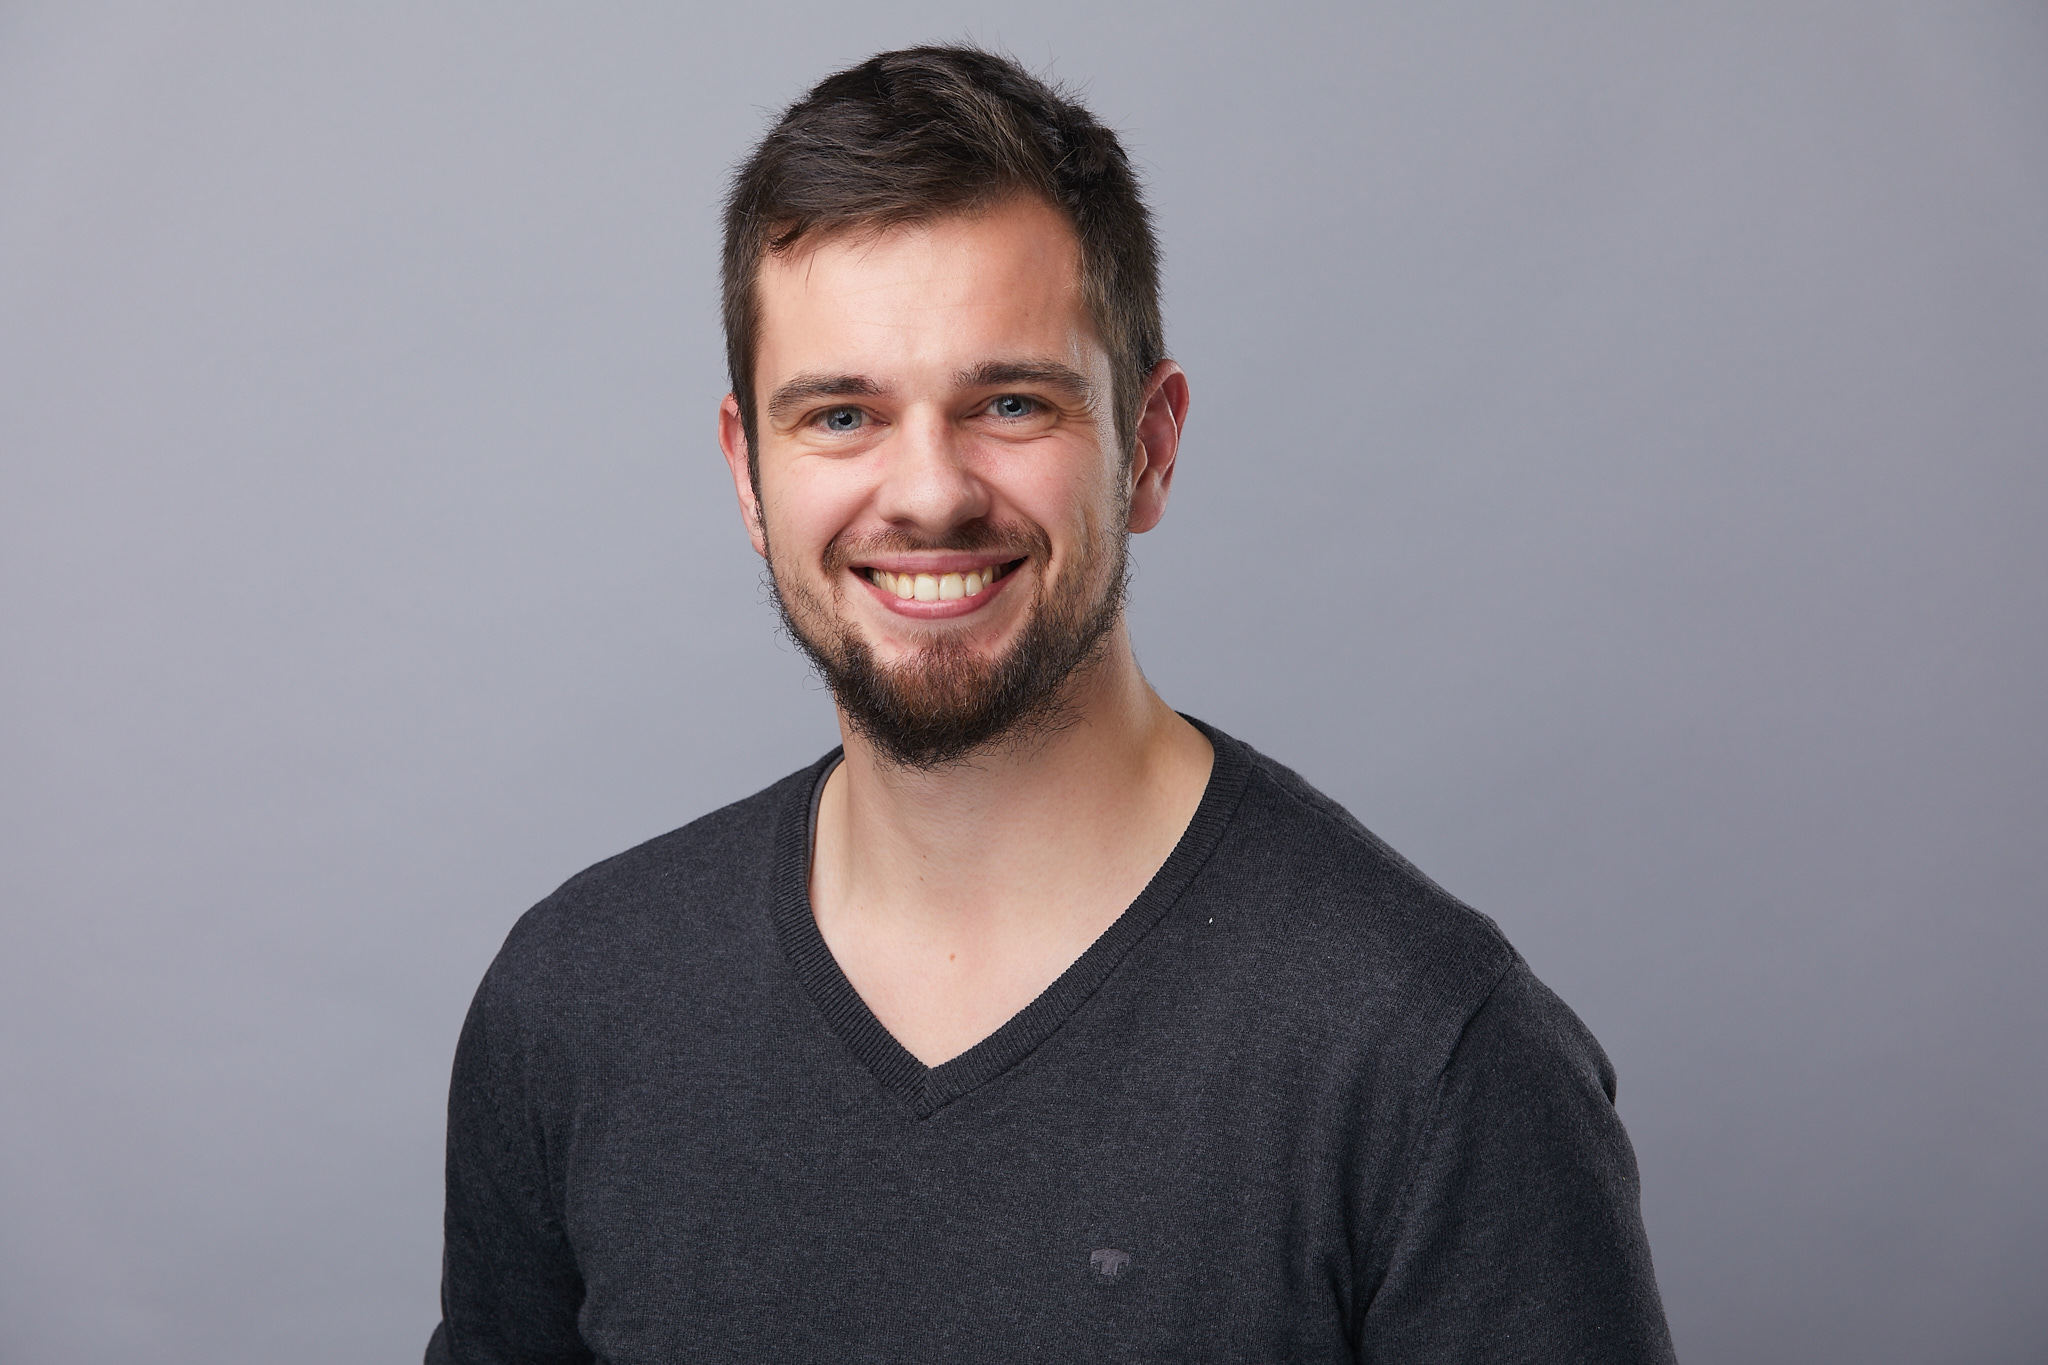
\includegraphics[width=\textwidth]{images/marc}
%%			\begin{tikzpicture}
%%			
%%			\node(marc) at (0,0){};
%%			
%%			\end{tikzpicture}
%		
%	\end{columns}
%\end{frame}

\begin{frame}
\frametitle{Background}

\begin{columns}
	\column{.75\textwidth}
%	Marc Rußwurm
%	\uncover<2->{
%		\begin{itemize}
%			\item born in raised in Bavaria, Germany.
%%			\item recently finished Master Geodesy \& Geoinformation @ TU Munich
%%			\item now started PhD @ TUM/DLR \\ Chair of Remote Sensing Technology
%%			\item member Computer Vision Research Group of my Chair
%		\end{itemize}
%	}
%	\uncover<3->{
%		\vspace{1em}
%		scientific interests
%		\begin{itemize}
%			\item multi-temporal EO
%%			\item time series with Recurrent Nets
%%			\item natural language processing $\rightarrow$ EO
%		\end{itemize}
%	}
%	\column{.25\textwidth}
%	\begin{tikzpicture}
%	
%	\node(marc) at (0,0){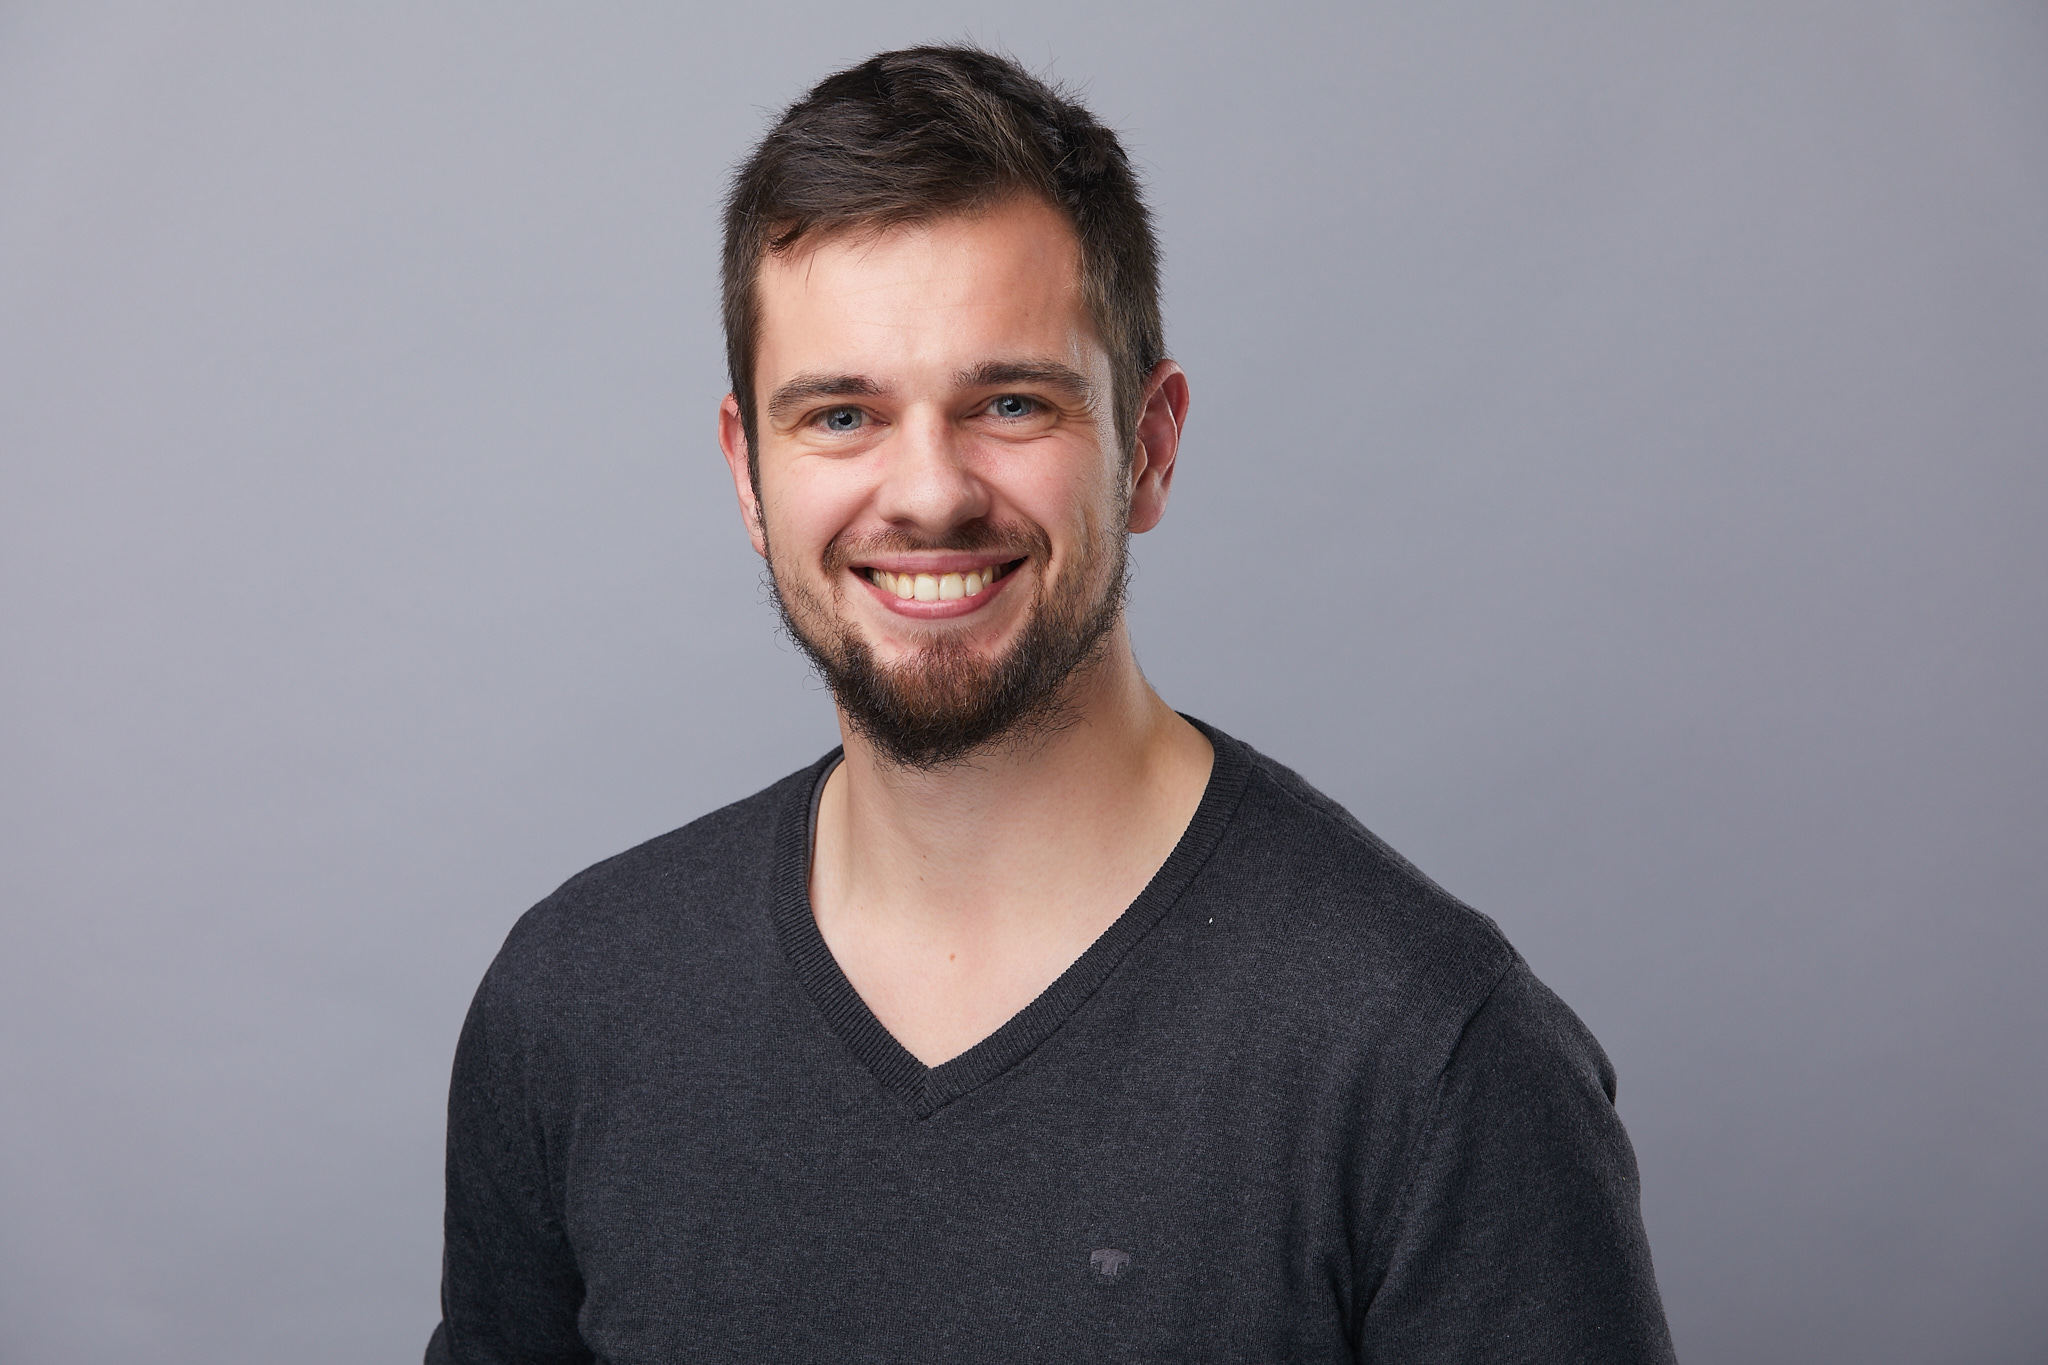
\includegraphics[width=\textwidth]{images/marc}};
%	
%	\end{tikzpicture}
	
\end{columns}

\tikzstyle{event} = [font=\small, text width=3.8cm, rounded corners=2em, inner sep=.7em]
\tikzstyle{date} = [font=\small, fill=white]
%
%\vspace{2em}

\begin{tikzpicture}[xscale=9, yscale=.85]

	\visible<1->{\node[anchor=east, label=Earth Observation] at (0,0){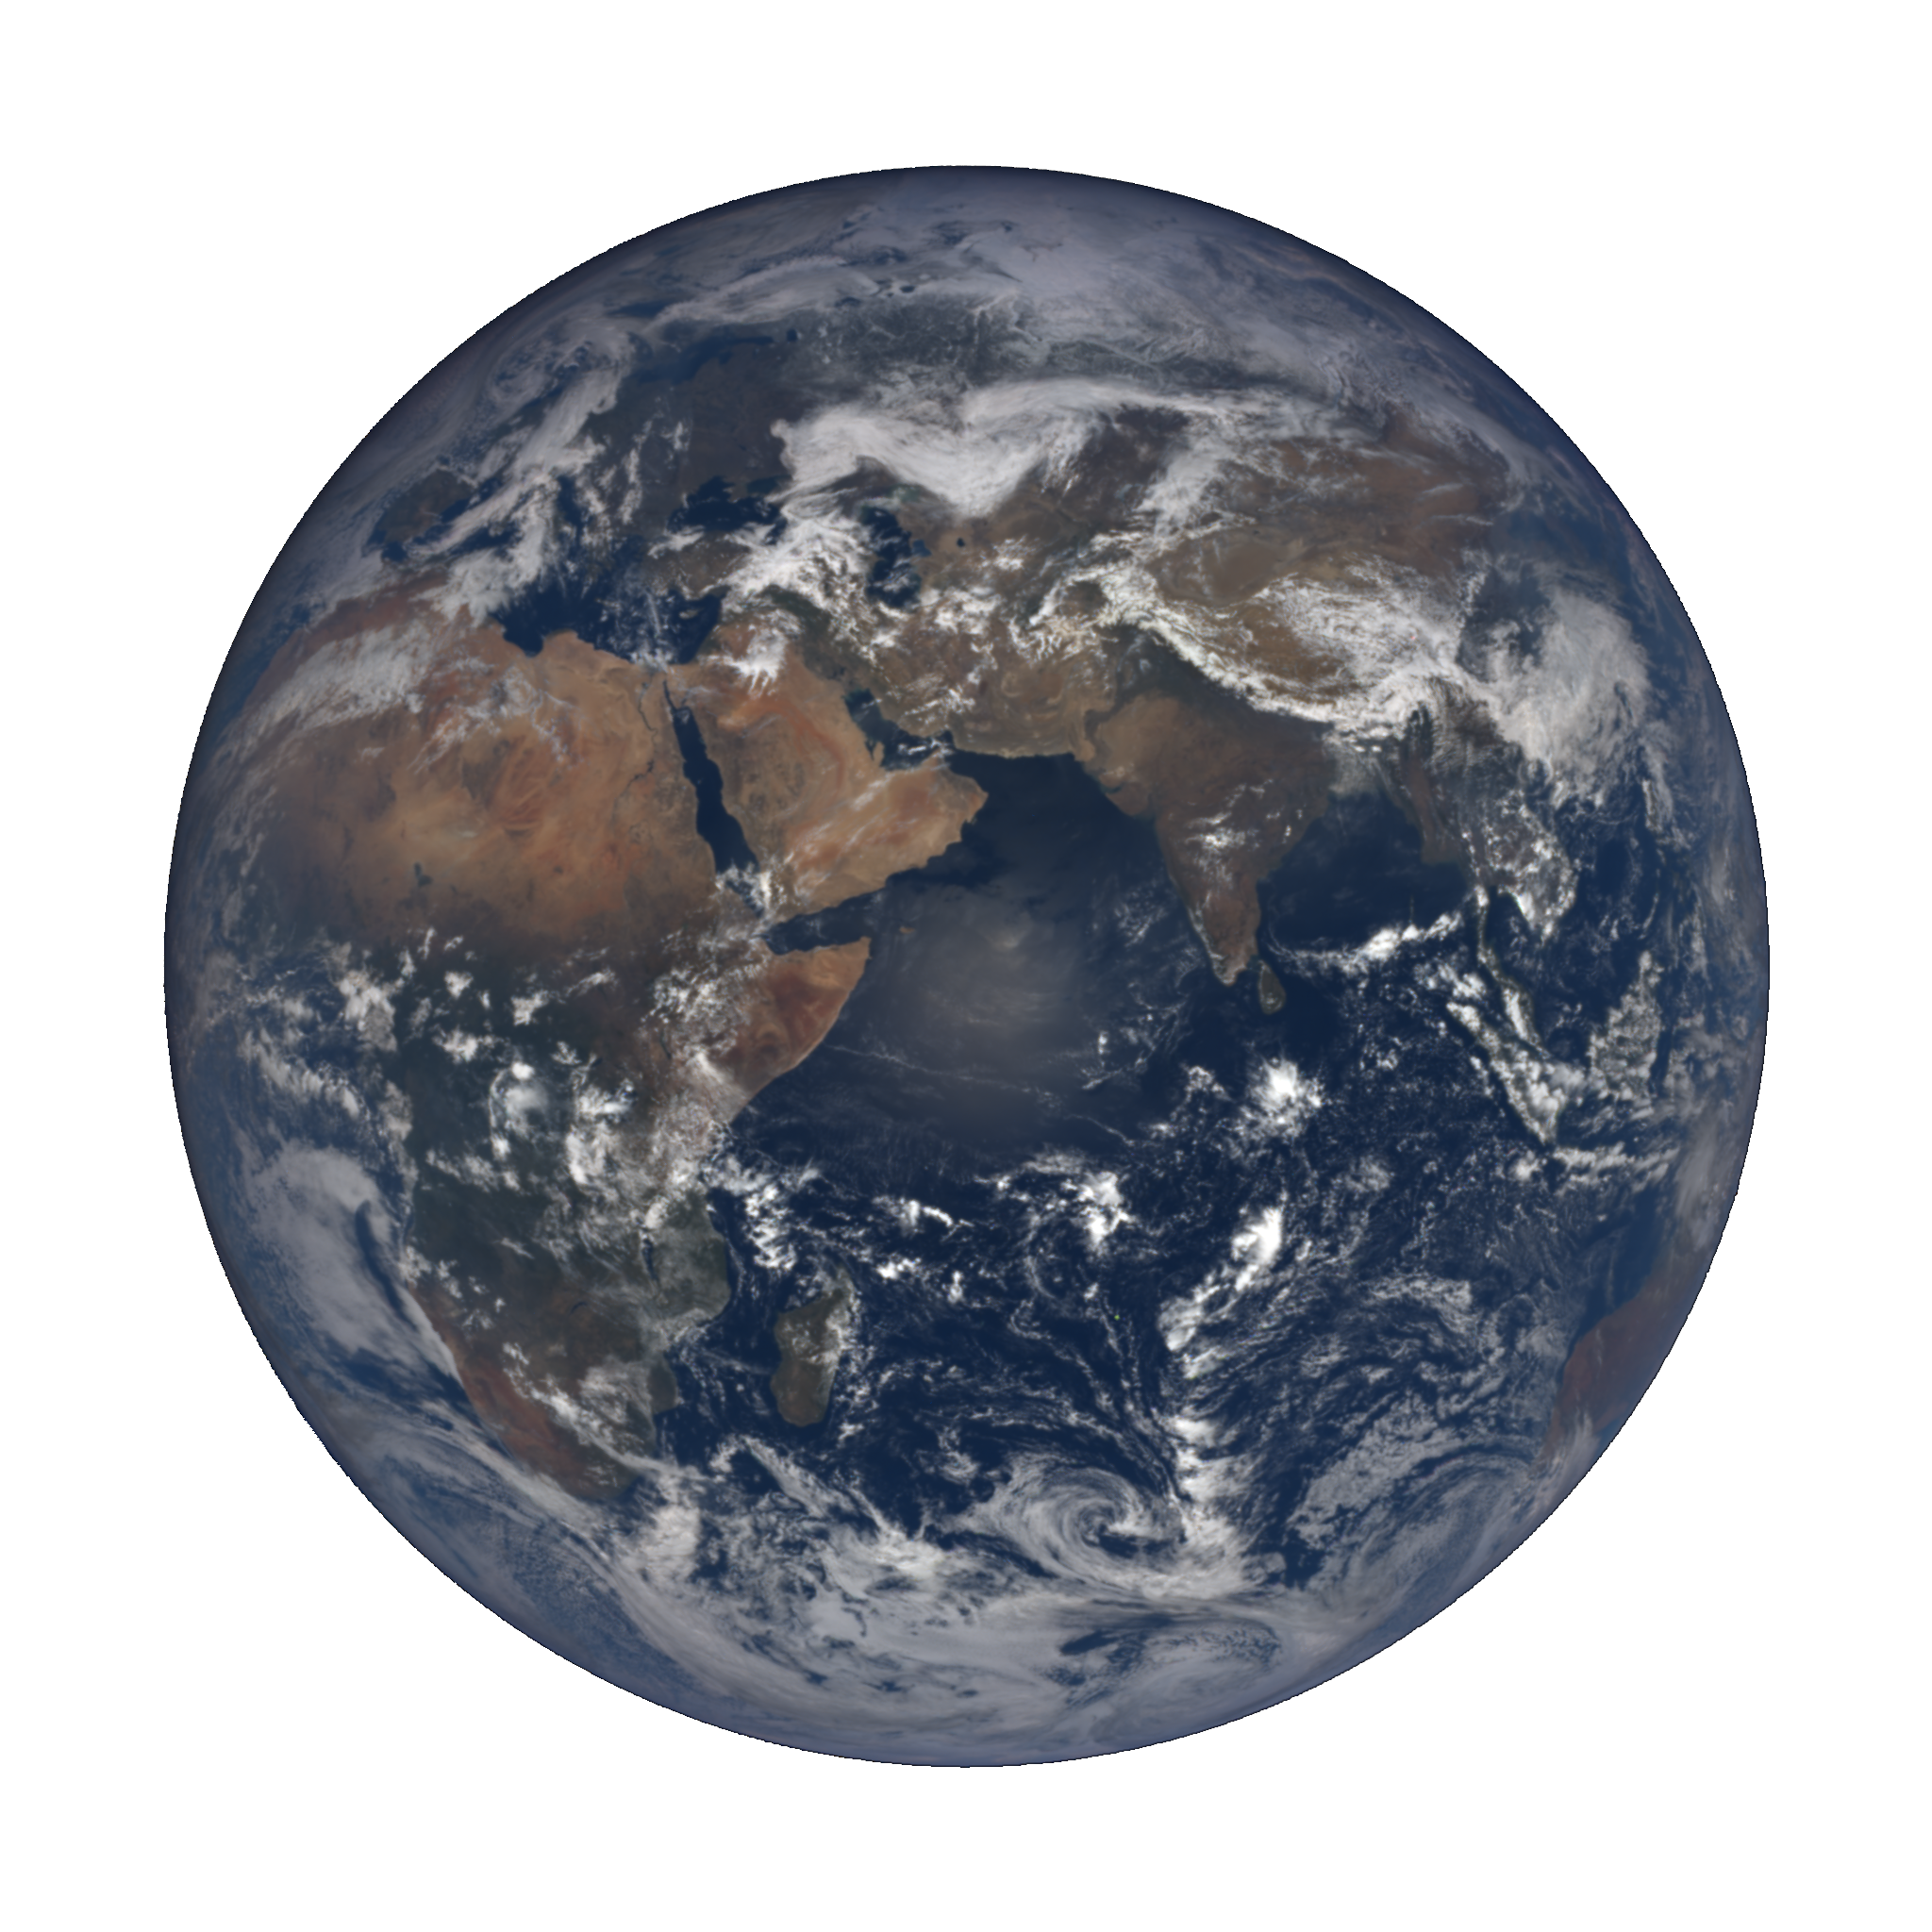
\includegraphics[width=3cm]{images/dscovrepic/epicw1}};}
	\visible<4->{\node[anchor=west, label=Machine Learning] at (1.1,0){\lfcn{.75}};}

	\node[event, fill=tumorange!50] at (.2,1) {2012-2018 \\ \textbf{Bachelor/Master} \\ Geodesy and Geoinformation};
	
	\visible<2->{\node[event, fill=tumbluelight] at (.3,-1) {2014 \\ Interned at University of Otago, NZ. \\ Geodata Visualization};}
	
	\visible<3->{\node[event, fill=tumbluelight] at (.1,-3) {2016 \\ Erasmus-interned at Polish Earth Observation Center \\ \textbf{Opium Poppy Detection}};}
	
	\visible<4->{\node[event, fill=tumorange!50] at (.7,2) {2018-2022 \\ \textbf{PhD} with Supervisor from Computer Vision \\ Multi-temporal Earth Observation};}
	
	\visible<5->{\node[event, fill=tumbluelight] at (.7,-3) {2018 \\ Participant \\ Frontier Developments Lab \\ Disaster Relief with \textbf{CNN data fusion}};}
	
	\visible<6->{\node[event, fill=tumbluelight] at (.8,-.5) {2019 \\ Research Stay IRISA Obelix Lab in France \\ \textbf{Early Classification of Time Series}};}
	
	
%	\draw (.8,6) node[date, above]{2019} -- node[event]{Research Stay \\ IRISA Obelix Lab in France} (.8,-3);
	
%	\draw (0,0)  node[left]{Earth Observation} -- node[at end, right]{Machine Learning} (1,0);
%	
%	\draw (.2,1) node[date, above]{2012-2018} -- node[event]{Studied B.Sc M.Sc Geodesy and Geoinformation} (.2,-1);
%
%	\draw (.2,2) node[date, above]{2014} -- node[event]{Interned at University of Otago, NZ. Geodata Visualization} (.2,-1);
%	
%	\draw (.1,3) node[date, above]{2016} -- node[event]{Erasmus-interned at Polish Earth Observation Center} (.1,-2);
%	
%	\draw (.7,4) node[date, above]{2018-2022} -- node[event]{PhD Supervisor in Computer Vision} (.7,-3);
%	
%	\draw (.6,5) node[date, above]{2018} -- node[event]{Participant in Frontier Developments Lab} (.6,-3);
%	 
%	\draw (.8,6) node[date, above]{2019} -- node[event]{Research Stay at IRISA Obelix Lab in France} (.8,-3);
	 
\end{tikzpicture}

\end{frame}



\newcommand{\focusdata}{{\color{tumblue}\textbf{data}~}}
\newcommand{\focusmethod}{{\color{tumorange}\textbf{method}~}}



\begin{frame}
	\frametitle{This Talk}
	
	\Large
	
	Organized in three parts
	
	\begin{description}
		\item[Part I] Overview Earth Observation
		\item[Part II] Research and Projects
		\item[Part III] Workshops and Programs around EO and ML
	\end{description}
\end{frame}

%{\setbeamercolor{background canvas}{bg=tumblue}
%	\begin{frame}[plain]
%	\vfill
%	\begin{center}
%		\Huge\color{tumwhite}
%		Remote Sensing Technology
%		
\includegraphics[width=5cm]{images/TUM-white}
%	\end{center}
%	
%	\vfill
%\end{frame}
%}





